\documentclass[11pt]{article}
\usepackage[margin=1in]{geometry}
\usepackage{amsmath,amssymb}
\usepackage{graphicx}
\usepackage{xcolor}
\usepackage{tikz}
\usetikzlibrary{arrows.meta, positioning}
\usepackage{enumitem}
\usepackage{parskip}
\usepackage[colorlinks=true, linkcolor=blue!50!black, citecolor=blue!50!black]{hyperref}

\definecolor{hdrblue}{RGB}{26,61,109}
\newcommand{\hsec}[1]{\section*{\color{hdrblue}#1}}
\newcommand{\hsub}[1]{\subsection*{#1}}

\title{\textbf{Flow-Matching Phantom Generation \& Interpolation}\\[4pt]
\large Project summary --- diffusion / flow-matching course project}
\author{}
\date{}

\begin{document}
\maketitle
\vspace{-1.2cm}

\hsec{What this project is}
The goal is to train a generative model over a dataset of 3D breast-phantom voxel scans,
then use that model to interpolate between two real phantoms --- not by blending their
voxels directly, but by inverting each phantom into the model's underlying noise
representation, interpolating there, and generating a new phantom back out. The idea is
that a smooth path through the model's internal representation should correspond to a
smooth, anatomically plausible morph between the two real examples, rather than a naive
crossfade.

\hsub{The data}
Each phantom is a 3D voxel volume ($K{=}26$ depth slices $\times\, H{=}128 \times W{=}128$),
where every voxel is one of 4 classes: background, insert, pillar, or lump (the class that
actually matters medically, and the rarest one). Raw voxel values $\{0,127,200,255\}$ are
remapped to class indices $\{0,1,2,3\}$. After removing double/triple-lump phantoms (out of
scope for this single-lump framing), 123 files across 40 case IDs remain, expanded to about
984 volumes via $8\times$ in-plane rotation augmentation on the training split.

\hsub{Why a generative model at all}
A direct voxel-space crossfade between two phantoms would just produce a physically
meaningless blur --- two lumps fading in and out of each other. Training a generative model
first means it learns a continuous, structured way to turn noise into valid-looking anatomy.
If that structure is smooth enough, moving smoothly through the model's noise representation
should also move smoothly through valid anatomy --- turning an interpolation problem in a
messy, discrete voxel space into an interpolation problem in a continuous space the model was
actually built to understand.

\hsec{The flow-matching process, from first principles}

\hsub{1. What we're trying to learn}
We have a data distribution we can sample from (real phantoms, one-hot encoded over the 4
classes so each voxel becomes a length-4 vector) but have no formula for. Call a sample from
it $x_1$. We also have a distribution we understand completely and can sample trivially:
standard Gaussian noise, $x_0 \sim \mathcal{N}(0, I)$, same shape as $x_1$. The goal is to
learn a transformation that turns noise into data --- concretely, a rule for continuously
moving a point from $x_0$ at ``time'' $t=0$ to $x_1$ at $t=1$.

\hsub{2. Pick a path between them}
The simplest possible path between two points is a straight line. For one paired sample
$(x_0, x_1)$, define the point along that line at time $t \in [0,1]$ as
\begin{equation}
x_t \;=\; (1-t)\,x_0 \;+\; t\,x_1. \label{eq:path}
\end{equation}
At $t=0$ this is exactly the noise; at $t=1$ it's exactly the real phantom; in between it's a
linear blend of the two. Differentiating Eq.~\eqref{eq:path} with respect to $t$ gives the
velocity a point moving along this line has at every instant --- and because the path is a
straight line, this velocity is simply constant along the whole path:
\begin{equation}
\frac{d x_t}{dt} \;=\; x_1 - x_0 \;=:\; v^*. \label{eq:vstar}
\end{equation}
$v^*$ is the target (or conditional) velocity for this specific pair: the same number for
every $t$ along this one path, but a different number for every different pair $(x_0,x_1)$ we
could have drawn.

\hsub{3. Learn a single velocity field that works for every pair}
We can't store a separate velocity for every possible $(x_0,x_1)$ pair --- there are
infinitely many. Instead we train a neural network $v_\theta(x,t)$ that takes any point $x$
and time $t$ and predicts what the velocity should be there, trained by regressing onto $v^*$
at randomly sampled points along randomly sampled paths:
\begin{equation}
\mathcal{L}(\theta) \;=\; \mathbb{E}_{\,t \sim U[0,1],\; x_0 \sim \mathcal{N}(0,I),\; x_1 \sim
p_{\text{data}}} \Big[\, \big\| v_\theta(x_t,t) - (x_1 - x_0) \big\|^2 \,\Big]. \label{eq:loss}
\end{equation}
At every training step: sample a real phantom $x_1$, sample fresh noise $x_0$, sample a
random $t$, form $x_t$ by Eq.~\eqref{eq:path}, run the network on $(x_t,t)$, and push its
output toward $x_1-x_0$. Over many such triples, the network is forced to learn a single,
shared velocity field consistent with every straight-line path it was shown, rather than
memorizing any one of them.

\hsec{Sampling, inversion, and the interpolation idea}

\hsub{4. Generating a new sample: integrate the field forward}
Once $v_\theta$ is trained, generating a new phantom means starting at pure noise
$x_0 \sim \mathcal{N}(0,I)$ at $t=0$ and numerically walking forward to $t=1$. Euler's method
splits $[0,1]$ into $n$ steps of size $\Delta t = 1/n$ and repeats
\begin{equation}
x_{t+\Delta t} \;=\; x_t + v_\theta(x_t,t)\,\Delta t. \label{eq:euler-fwd}
\end{equation}
After $n$ steps this produces a generated $\hat x_1$ --- a continuous, 4-channel volume.
Taking the argmax over the 4 channels at every voxel turns it back into a discrete label
volume that can be rendered. This is what \texttt{ode.py}'s \texttt{sample()} does;
\texttt{n\_steps} trades accuracy for compute.

\hsub{5. Inverting a real phantom: integrate the field backward}
The learned field also lets us go the other way. Given a real phantom $x_1$, integrating the
same equation backward from $t=1$ to $t=0$,
\begin{equation}
x_{t-\Delta t} \;=\; x_t - v_\theta(x_t,t)\,\Delta t, \label{eq:euler-bwd}
\end{equation}
recovers an approximate noise pre-image $\hat x_0$ for it. If the network has learned the
field well, integrating forward from $\hat x_0$ should reconstruct something very close to
the original $x_1$. We verified this directly with a round-trip test (Section~6) and measured
96--99\% voxel agreement at 50 integration steps.

\hsub{6. The actual interpolation idea}
To morph between two real phantoms A and B: invert both to get $\hat x_0^A$ and
$\hat x_0^B$, interpolate between these two noise representations at mixing fraction
$\alpha \in [0,1]$, then integrate the interpolated point forward to $t=1$. A plain linear
blend of two Gaussian vectors isn't right, though (Section~4.3 makes this precise): spherical
interpolation (slerp) moves along the great-circle arc between the two vectors instead,
preserving their norm the whole way,
\begin{equation}
\mathrm{slerp}(a,b,\alpha) \;=\; \frac{\sin\big((1-\alpha)\theta\big)}{\sin\theta}\,a \;+\;
\frac{\sin(\alpha\theta)}{\sin\theta}\,b, \qquad \theta = \arccos\!\left(\frac{a\cdot b}{\|a\|\,\|b\|}\right).
\label{eq:slerp}
\end{equation}
The full pipeline per $\alpha$ step: invert A and B to noise, slerp between them at that
$\alpha$, integrate forward through $v_\theta$, argmax to a label volume, render. The
noise-interpolation variant skips inversion and slerps between two directly-sampled Gaussian
points instead.

\hsec{Dimensionality and distributions, in detail}
This section works through exactly what shape and distribution every object in the pipeline
has, because the interpolation failure we diagnose in Section~6 turns out to be a direct
consequence of these numbers, not of a bug.

\hsub{4.1 Exact shapes}
Every one of $x_0$, $x_1$, $x_t$, $v_\theta(x_t,t)$, and $v^*$ has the identical shape: 4
channels $\times$ 26 depth slices $\times$ 128 $\times$ 128. Flattened into a single vector,
that is a space of dimension
\begin{equation}
d \;=\; 4 \times 26 \times 128 \times 128 \;=\; 1{,}703{,}936. \label{eq:dim}
\end{equation}
Every noise sample, every real phantom, every intermediate $x_t$, and the noise pre-image
$\hat x_0$ from inversion are all points in this same $d \approx 1.7$ million dimensional
space. There is no bottleneck anywhere in this architecture --- see 4.4.

\hsub{4.2 The distributions at each stage}
$x_0 \sim \mathcal{N}(0, I_d)$ by construction: every coordinate is an independent standard
Gaussian. $x_1$ is not continuous at all: each voxel is constrained to be one of the 4
one-hot corners of a simplex, so $x_1$ lives on a discrete, highly constrained subset of
$\mathbb{R}^d$ (only a tiny sliver of which corresponds to real anatomy). For a \emph{fixed}
real phantom $x_1$, Eq.~\eqref{eq:path} is an affine function of the Gaussian $x_0$, so $x_t$
conditioned on $x_1$ is itself Gaussian:
\begin{equation}
x_t \mid x_1 \;\sim\; \mathcal{N}\big(t\,x_1,\ (1-t)^2 I_d\big). \label{eq:conditional-path}
\end{equation}
This collapses to $\mathcal{N}(0,I_d)$ at $t=0$ and to a point mass at $x_1$ at $t=1$, exactly
as expected. Averaging Eq.~\eqref{eq:conditional-path} over the whole training distribution of
real phantoms gives the true \emph{marginal} distribution the network sees $x_t$ drawn from
at every $t$:
\begin{equation}
p_t(x) \;=\; \mathbb{E}_{x_1 \sim p_{\text{data}}}\Big[\, \mathcal{N}\big(x;\ t\,x_1,\ (1-t)^2 I_d\big) \,\Big],
\label{eq:marginal-path}
\end{equation}
a continuous mixture of Gaussians with one mixture component centered at $t \cdot x_1$ for
every real phantom in the data.

\hsub{4.3 High-dimensional geometry: why slerp and not a linear blend}
\textbf{Intuition first.} A noise sample is $d\approx 1.7$ million independent random numbers,
one per voxel-channel. No individual number is predictable. But its \emph{length} --- distance
from the origin, computed the ordinary way (square every coordinate, add them all up, take the
square root) --- is a sum of 1.7 million independent random pieces. Individually each piece is
random, but adding up millions of independent random things makes the total extremely
predictable: it is the same reason a casino always turns a profit even though any single spin
of the wheel is random. So even though no single coordinate of a noise vector can be predicted,
its overall length can be, almost exactly. That length is what the formulas below pin down as
$\approx 1305$.

Now picture two arrows of equal length in ordinary 3D space, pointing in different directions.
Add them tip-to-tail and take the midpoint: that midpoint arrow is \emph{shorter} than either
original, because the two arrows form a narrow ``V'' and the midpoint sits inside it, closer to
the vertex. Only if the two arrows point in exactly the same direction does averaging preserve
the length. In a space with 1.7 million dimensions, two random directions are essentially
always close to \emph{perpendicular} to each other, and averaging two equal-length,
perpendicular arrows shrinks the result by a fixed factor of $1/\sqrt{2}\approx 0.71$. That is
the entire reason a linear blend of two noise vectors comes out too short --- it is just this
``V'' shrinkage, happening in a space too big to visualize.

Spherical interpolation (slerp) avoids the shrinkage differently: instead of cutting straight
through the middle of the ``V'' (which is what shrinks the length), it walks along the surface
of the sphere connecting the two points --- like flying from New York to London along the
Earth's curved surface instead of drilling straight through the planet's core. Every point on
that curved flight path is still exactly the same distance from the Earth's center as New York
and London are. Slerp's output is always the correct length, for every mixing fraction, no
matter what.

\textbf{Now the same argument with the numbers.} For $X \sim \mathcal{N}(0,I_d)$, $\|X\|^2$
follows a chi-squared distribution with $d$ degrees of freedom: mean $d$, variance $2d$. Using
$d = 1{,}703{,}936$ from Eq.~\eqref{eq:dim},
\begin{equation}
\mathbb{E}\big[\|X\|^2\big] = d \approx 1{,}703{,}936, \qquad
\mathbb{E}\big[\|X\|\big] \approx \sqrt{d} \approx 1305.4. \label{eq:norm-mean}
\end{equation}
By the delta method, $\mathrm{Var}(\|X\|) \approx \mathrm{Var}(\|X\|^2)/(4d) = 2d/4d = 1/2$,
i.e.\ $\mathrm{SD}(\|X\|) \approx 0.71$ --- a constant, \emph{not growing with $d$}. The relative
fluctuation of the norm is therefore about $0.71/1305.4 \approx 0.05\%$: essentially every
Gaussian sample lands within a hair's width of the same radius, on a thin ``shell'' around the
origin (the ``casino'' argument above, made precise). This is the concentration-of-measure
phenomenon.

Now take two independent samples $a,b \sim \mathcal{N}(0,I_d)$ and average them,
$m = (a+b)/2$. Since $a,b$ are independent, $m \sim \mathcal{N}(0, I_d/2)$, so by the same
formula
\begin{equation}
\mathbb{E}\big[\|m\|\big] \approx \sqrt{d/2} \approx 923.1, \label{eq:norm-mid}
\end{equation}
about $70.7\% \approx 1/\sqrt{2}$ of the typical shell radius $1305.4$ --- exactly the ``V''
shrinkage described above, now with a number attached. The midpoint of two random Gaussian
samples reliably lands at a norm around $923$, nowhere near the shell (radius $\approx 1305$)
that Gaussian noise --- and every noise pre-image the model was actually trained near --- lives
on. A linear blend is handing the network an input from a part of space it essentially never
sees. Spherical interpolation avoids this: for $\|a\|=\|b\|=r$, Eq.~\eqref{eq:slerp} gives
$\|\mathrm{slerp}(a,b,\alpha)\| = r$ exactly, for every $\alpha$ --- the interpolated point
stays on the same shell as the two endpoints by construction.

\textbf{What slerp does and doesn't guarantee.} It is worth being precise about what this
buys us, because it is easy to overstate. Slerp guarantees that $z_\alpha$ sits at the correct
\emph{angular} position between $\hat x_0^A$ and $\hat x_0^B$ on the sphere --- at $\alpha=0.5$
it is, by literal construction, the exact geographic midpoint of the flight path between them.
That much is not an assumption; it follows directly from the formula. What it does \emph{not}
guarantee is that this midpoint \emph{decodes} to an anatomy that is ``in between'' phantom A
and phantom B. The network is a smooth, continuous function, so it changes gradually as you
slide along the arc from A to B --- but gradual is not the same as meaningful. Continuity only
forbids sudden jumps; it does not forbid the decoded shape gradually tearing into a fragmented
mess and back. The network was only ever taught the translation from noise-sphere position to
anatomy \emph{at} $\hat x_0^A$ and \emph{at} $\hat x_0^B$ (Section~4.5): nobody ever told it
what the geographic midpoint of that specific flight path should mean. Slerp guarantees we ask
the network a fair, correctly-scaled question; it does not guarantee the network knows the
answer. That gap --- between asking a fair question and getting a meaningful answer --- is
precisely the failure diagnosed in Section~6, and precisely what $t_{\text{mid}}$ (Section~7)
targets: moving the question to a place closer to territory the network actually studied.

\hsub{4.4 Compression: what flow matching does \emph{not} do}
A VAE compresses data through a bottleneck --- typically a few hundred to a few thousand
numbers --- and an explicit KL-divergence term during training forces that bottleneck's
distribution toward a simple, smooth prior. That explicit pressure to compress is exactly what
makes VAE latent spaces organize into something that interpolates nicely: with no room to
memorize per-example detail, the model is forced to generalize.

Flow matching does not compress at all. From Eq.~\eqref{eq:dim}, $x_0$ lives in the
\emph{same} $d\approx 1.7$ million dimensional space as the data --- there is no bottleneck,
and nothing in the loss (Eq.~\eqref{eq:loss}) ever pushes the noise space to be smoothly
\emph{organized} as a whole. The loss only ever asks the network to get one straight-line path
right at a time. That is a deliberate trade-off (no compression means no lost detail, which is
why diffusion/flow models produce sharper samples than typical VAEs), but it is also exactly
why individual inversion is excellent while interpolation between two different phantoms'
noise pre-images is not: nothing in training ever touches the region \emph{between} two
different paths.

\hsub{4.5 How sparse is the training data in this space?}
The training set has on the order of $10^3$ augmented volumes (984, from 8$\times$ rotation
augmentation of the 40 case IDs). Those are $10^3$ points scattered across a space of
dimension $d \approx 1.7\times 10^6$. There is no meaningful sense in which $10^3$ points can
densely cover a $1.7$-million-dimensional space; the network only ever gets direct signal
along the specific handful of straight lines it was shown, and has to extrapolate everywhere
else. This is the quantitative version of the ``uneven coverage'' explanation in Section~6.

\hsub{4.6 Why the rendered noise pre-image ($z$) looks the wrong size}
Real phantom voxels are drastically imbalanced: measured directly from the data,
\begin{equation}
\text{background} = 50.8\%,\quad \text{insert} = 48.0\%,\quad
\text{pillar} = 0.32\%,\quad \text{lump} = 0.94\%. \label{eq:class-balance}
\end{equation}
That imbalance is a property of real anatomy, not of the representation. A noise pre-image
$\hat x_0$, however, is close to i.i.d.\ Gaussian per channel per voxel; by symmetry, each of
the 4 channels wins the per-voxel argmax with probability $1/4 = 25\%$. So when we render
$\hat x_0$ using the same argmax-then-mesh-extract pipeline used for real data, the lump
channel --- which wins about $0.94\%$ of voxels in real anatomy --- suddenly wins about
\emph{25\%} of all voxels, roughly a $26\times$ increase in footprint. That is exactly why the
``$z$'' panel in Figure~\ref{fig:inversion0} shows a lump region far larger than any real
phantom's, and why it extends all the way to the edges of the volume: real data always has
background surrounding the anatomy acting as a boundary, and noise has no such boundary.

\hsec{Loss functions: plain MSE, then class-weighted MSE}

\hsub{The starting point: unweighted per-voxel MSE}
The loss in Eq.~\eqref{eq:loss} is a per-voxel, per-channel squared error averaged uniformly
over every voxel and all 4 channels. It has no notion of ``class'': a lump voxel is worth
exactly as much as a background voxel in the average.

\hsub{Why that's a problem here}
From Eq.~\eqref{eq:class-balance}, background and insert together make up almost the entire
voxel count. A model can get the loss almost perfectly low just by nailing those two classes,
while being essentially wrong about the lump with barely any effect on the reported loss. This
matched what we observed directly: the overall phantom shape was learned solidly and
consistently, while the lump was inconsistent --- present, shrunk, or missing across training
checkpoints and across repeated samples from the same fixed noise seed.

\hsub{The fix that was tried: class-weighted MSE}
Multiply the squared error at each voxel by a weight depending on its true class, before
averaging:
\begin{equation}
\mathcal{L}_{\text{weighted}}(\theta) \;=\; \mathbb{E}\left[\, \frac{1}{C\cdot D}
\sum_{c=1}^{C} w_c \sum_{\text{voxels}} \big(v_\theta - v^*\big)^2_{c,\text{voxel}} \,\right],
\label{eq:weighted-loss}
\end{equation}
with $w_c$ set to the square root of inverse class frequency, normalized so background$=1$:
\begin{equation}
w = (1.0,\ 1.03,\ 12.57,\ 7.36) \quad \text{for (background, insert, pillar, lump).}
\label{eq:weights}
\end{equation}
Square root rather than raw inverse frequency deliberately: raw inverse frequency would give
pillar $\approx 158\times$ the weight of background, risking letting a handful of rare voxels
dominate the gradient and destabilize training.

\hsub{What actually happened}
Plain unconditional generation looked about the same, maybe marginally more consistent about
including a lump. Real-phantom interpolation got noticeably \emph{worse}: instead of a clean
shape with a duplicated lump (the old failure mode), the interpolated shape itself started
tearing and fragmenting. Section~6 works out why.

\hsec{Diagnostics: visualizing and ruling things out}

\hsub{Visualizing the round trip directly}
Beyond the voxel-agreement number, we built a script
(\texttt{flow\_model/visualize\_inversion.py}) that inverts a real, randomly-rotated
(augmented) validation phantom to its noise pre-image and re-generates it, logging a
before~$\to$~$z$~$\to$~after figure to Weights \& Biases. Figure~\ref{fig:inversion0} shows one
example (checkpoint: 1000-epoch, class-weighted loss). The reconstruction (``after'') closely
matches the original (``before''), at 92.7\% voxel agreement --- consistent with the
round-trip numbers measured earlier. The middle panel (``$z$'') is explained in
Section~4.6: it is not a bug that it looks large and boxy, that is the expected appearance of
argmax'd near-Gaussian noise given the real class imbalance.

\begin{figure}[h]
\centering
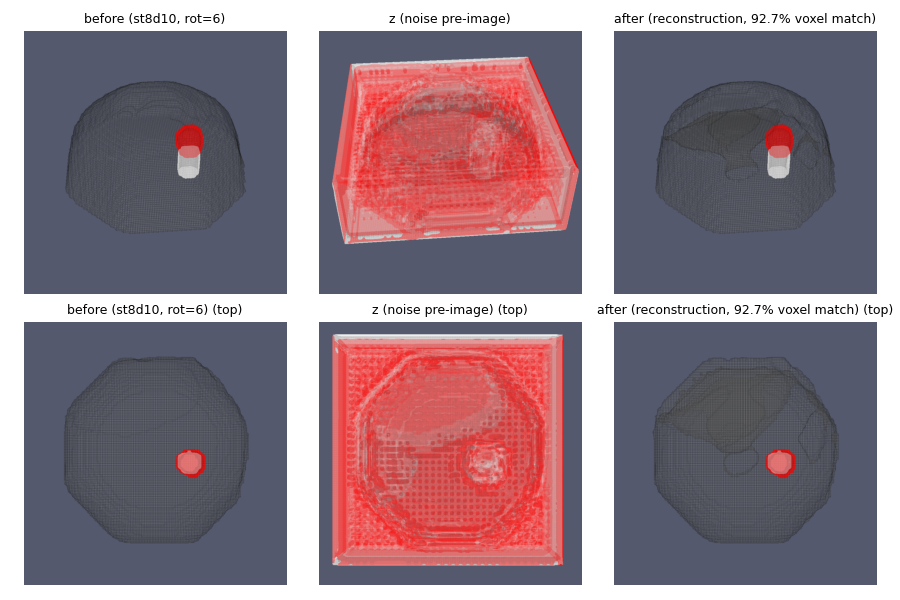
\includegraphics[width=\textwidth]{imgs/summary/inversion_example0.png}
\caption{Before (real, rotated phantom) $\to$ $z$ (inverted noise pre-image) $\to$ after
(re-generated from $z$). Top row: default angled view. Bottom row: top-down view. Checkpoint:
1000-epoch, class-weighted loss.}
\label{fig:inversion0}
\end{figure}

\hsub{Ruling out bad inversion}
The first suspect for the broken interpolation was inversion itself. We tested this with a
round-trip check (invert a real phantom, regenerate, measure voxel agreement with the
original): 96--99\% agreement at 50 steps, on both the original and the class-weighted
checkpoints. Inversion of a single phantom is excellent either way --- this rules out
``inversion is unreliable'' as the explanation.

\hsub{Ruling out numerical/discretization error}
Next suspect: maybe 50 ODE integration steps isn't enough resolution once the field is
sharper. Rerunning the same interpolation with 150 steps instead of 50 produced essentially
the same broken shape --- same tear, same scattered fragments, in nearly the same positions.
A genuine discretization error would be expected to improve with $3\times$ more resolution;
this didn't, which rules out step count as the cause.

\hsub{What's actually going on}
Section~4.4--4.5 give the quantitative version of this: flow matching only ever trains on
individual straight-line paths, each from one random noise sample to one specific real
phantom, in a space so large ($d\approx 1.7\times10^6$) that $\sim\!10^3$ training examples
cover only a vanishing sliver of it. Nothing in training constrains what should happen at
points between two different phantoms' separate paths, and at $t=0$ (pure noise) that
neighborhood is the least-constrained region in the entire space. Figure~\ref{fig:interp-broken}
shows a representative example: the two endpoints (blue/orange borders) are clean, and the
``actual'' generated lump position (green $\times$) happens to land almost exactly on the naive
linearly ``expected'' position (red star) this time --- but the interpolated anatomy itself
still visibly warps, growing extra bumps and a few disconnected floating specks that are not
present in either endpoint. Centroid position and overall anatomical quality are two separate
things the model can get wrong independently, and this example shows the latter failing even
when the former happens to succeed.

\begin{figure}[h]
\centering
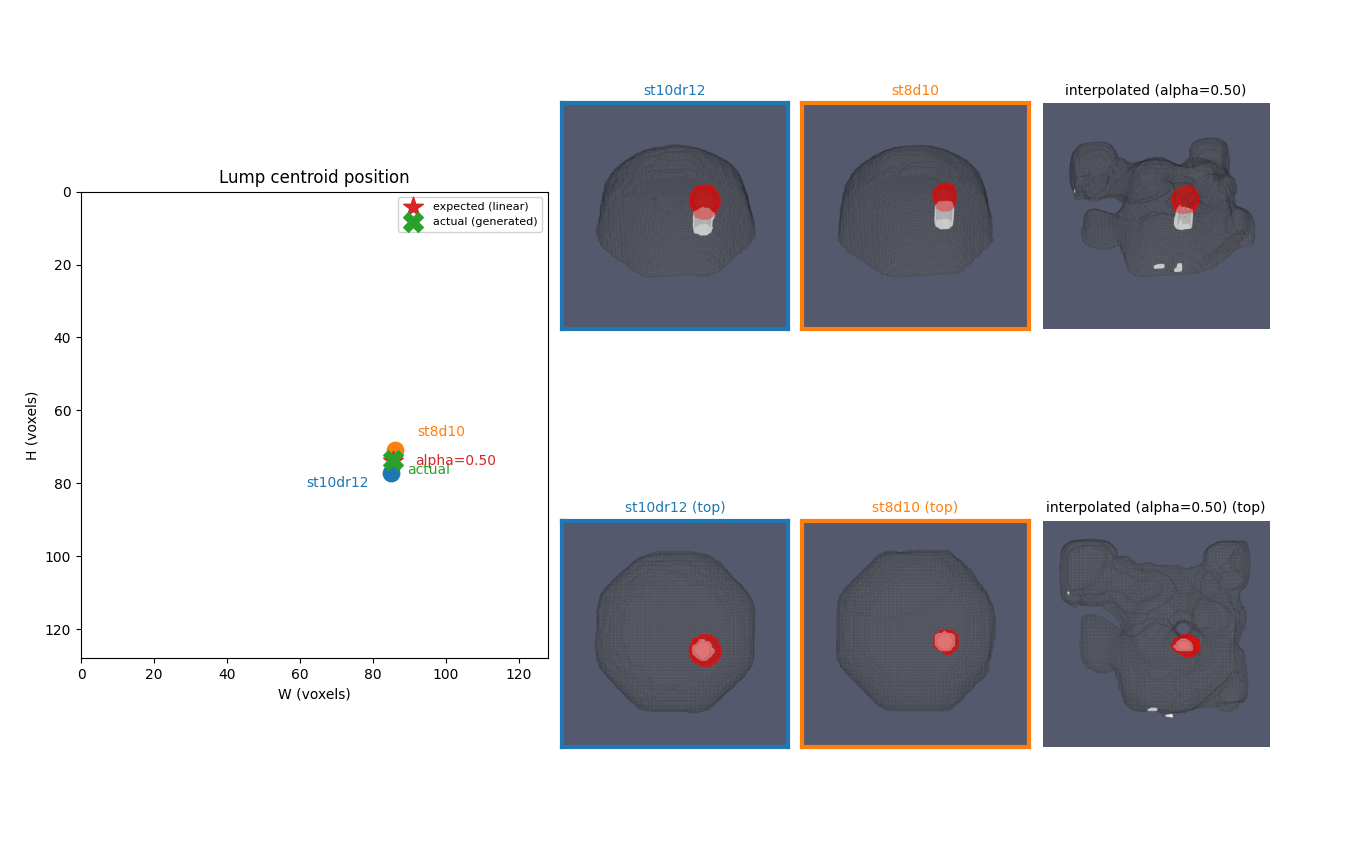
\includegraphics[width=\textwidth]{imgs/summary/interp_broken_example.png}
\caption{A representative real-phantom interpolation (pair: \texttt{st10dr12}
$\leftrightarrow$ \texttt{st8d10}, $\alpha=0.5$). Left: lump-centroid schematic, showing the
naive linearly-expected position (red star) versus what the model actually generated (green
$\times$) --- close this time. Right: renders of both endpoints and the interpolated result;
note the extra bumps and small disconnected specks that appear in the interpolated anatomy but
in neither endpoint.}
\label{fig:interp-broken}
\end{figure}

We also checked 10 different real-phantom pairs at the same $\alpha$ values directly: the
failure is inconsistent rather than universal --- a couple of pairs interpolated cleanly on
both counts (centroid position \emph{and} anatomy), some (like Figure~\ref{fig:interp-broken})
get the centroid right but still distort the anatomy, and others miss badly on both. That
matches uneven coverage: some pairs' inverted noise points happen to sit near a well-covered
part of the space, most don't, and it isn't simply a function of how far apart the two
phantoms' lumps start out.

\hsec{Where things stand, and the proposed next step}

\hsub{Working}
Unconditional generation from noise: solid, consistent anatomy, lump present in most fixed
evaluation seeds. Inversion of a single real phantom back to noise: highly accurate. The
overall pipeline mechanics all run end-to-end without errors.

\hsub{Not yet working}
Real-phantom interpolation via invert / slerp / forward-integrate is unreliable --- it works
for some pairs and produces torn, fragmented anatomy for most others. Neither more training
epochs, class-weighting the loss, nor more ODE integration steps fixed this.

\hsub{Proposed next step: interpolate at partial inversion ($t_{\text{mid}}$)}
The core idea: don't fully invert either phantom all the way to $t=0$. Only invert
\emph{partway}, to some intermediate $t_{\text{mid}} > 0$ (e.g.\ 0.2--0.3), interpolate the two
phantoms' partial trajectories \emph{there}, and integrate forward the remaining distance from
$t_{\text{mid}}$ to $t=1$. Figure~\ref{fig:tmid} makes this mechanical: the top row is the
current (broken) approach, the bottom row is the proposal.

\begin{figure}[h]
\centering
\resizebox{\textwidth}{!}{%
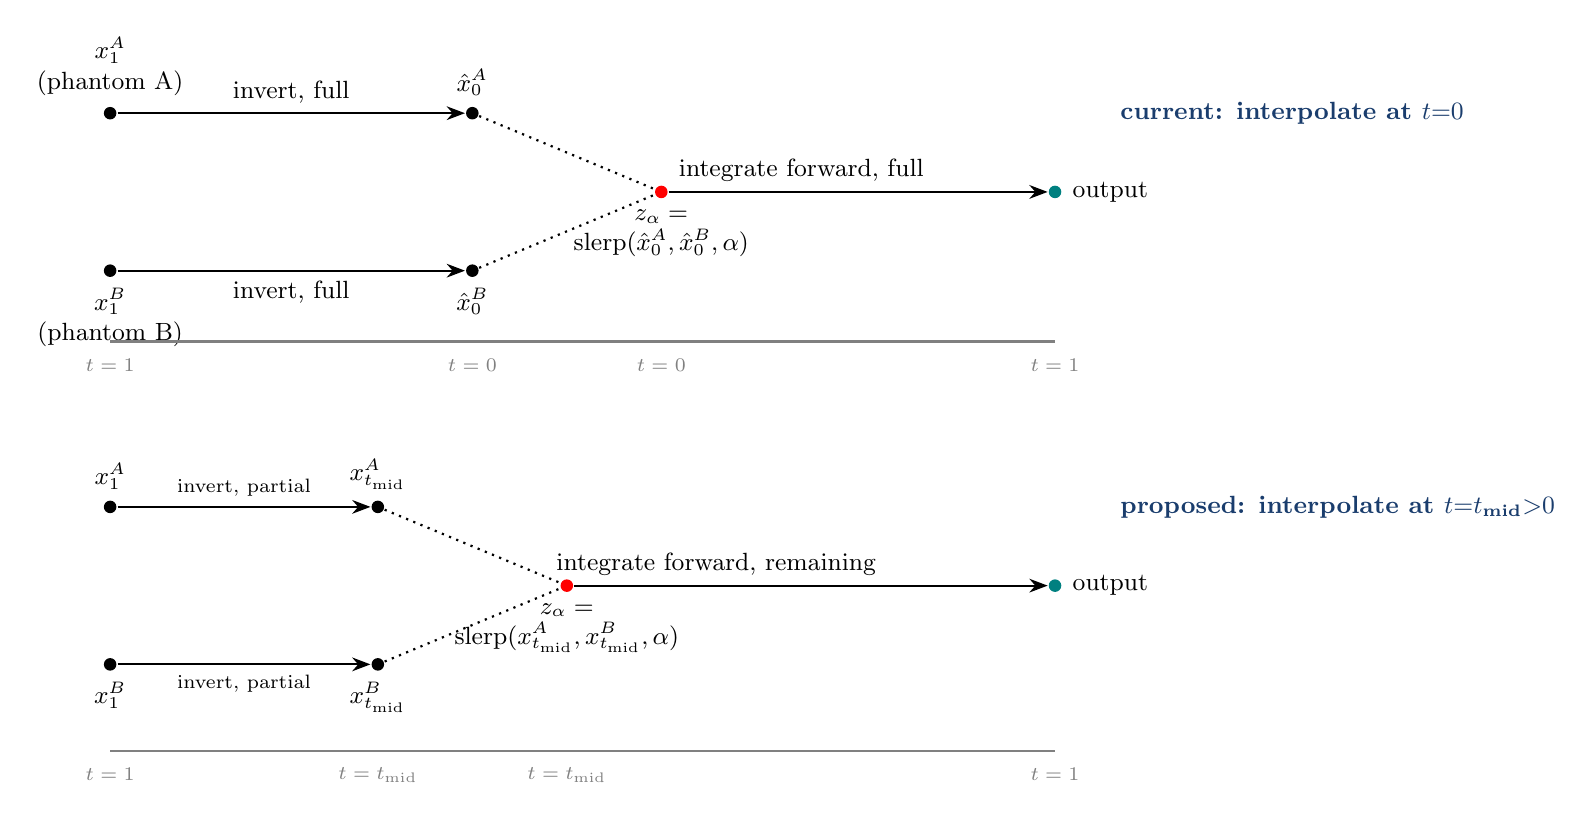
\begin{tikzpicture}[
  >=Stealth, thick,
  ptnode/.style={circle, fill, inner sep=1.6pt},
  every node/.style={font=\small}
]
% ---- Row 1: current approach (t_mid = 0) ----
\node[ptnode, label={[align=center]above:{$x_1^A$\\(phantom A)}}] (A1) at (0,3.2) {};
\node[ptnode, label={[align=center]below:{$x_1^B$\\(phantom B)}}] (B1) at (0,1.2) {};
\node[ptnode, label=above:{$\hat x_0^A$}] (A0) at (4.6,3.2) {};
\node[ptnode, label=below:{$\hat x_0^B$}] (B0) at (4.6,1.2) {};
\node[ptnode, fill=red, label={[align=center]below:{$z_\alpha =$\\$\mathrm{slerp}(\hat x_0^A, \hat x_0^B,\alpha)$}}] (Z1) at (7,2.2) {};
\node[ptnode, fill=teal, label=right:{output}] (O1) at (12,2.2) {};
\draw[->] (A1) -- node[above, pos=0.5]{invert, full} (A0);
\draw[->] (B1) -- node[below, pos=0.5]{invert, full} (B0);
\draw[dotted] (A0) -- (Z1);
\draw[dotted] (B0) -- (Z1);
\draw[->] (Z1) -- node[above, pos=0.35]{integrate forward, full} (O1);
\node[anchor=west, color=hdrblue] at (12.7,3.2) {\textbf{current: interpolate at $t{=}0$}};

% timeline for row 1
\draw[-, gray] (0,0.3) -- (12,0.3);
\node[gray, font=\scriptsize] at (0,0.0) {$t=1$};
\node[gray, font=\scriptsize] at (4.6,0.0) {$t=0$};
\node[gray, font=\scriptsize] at (7,0.0) {$t=0$};
\node[gray, font=\scriptsize] at (12,0.0) {$t=1$};

% ---- Row 2: proposed approach (t_mid > 0) ----
\node[ptnode, label=above:{$x_1^A$}] (A1b) at (0,-1.8) {};
\node[ptnode, label=below:{$x_1^B$}] (B1b) at (0,-3.8) {};
\node[ptnode, label=above:{$x_{t_{\text{mid}}}^A$}] (A0b) at (3.4,-1.8) {};
\node[ptnode, label=below:{$x_{t_{\text{mid}}}^B$}] (B0b) at (3.4,-3.8) {};
\node[ptnode, fill=red, label={[align=center]below:{$z_\alpha =$\\$\mathrm{slerp}(x_{t_{\text{mid}}}^A, x_{t_{\text{mid}}}^B,\alpha)$}}] (Z2) at (5.8,-2.8) {};
\node[ptnode, fill=teal, label=right:{output}] (O2) at (12,-2.8) {};
\draw[->] (A1b) -- node[above, pos=0.5, font=\scriptsize]{invert, partial} (A0b);
\draw[->] (B1b) -- node[below, pos=0.5, font=\scriptsize]{invert, partial} (B0b);
\draw[dotted] (A0b) -- (Z2);
\draw[dotted] (B0b) -- (Z2);
\draw[->] (Z2) -- node[above, pos=0.3]{integrate forward, remaining} (O2);
\node[anchor=west, color=hdrblue] at (12.7,-1.8) {\textbf{proposed: interpolate at $t{=}t_{\text{mid}}{>}0$}};

\draw[-, gray] (0,-4.9) -- (12,-4.9);
\node[gray, font=\scriptsize] at (0,-5.2) {$t=1$};
\node[gray, font=\scriptsize] at (3.4,-5.2) {$t=t_{\text{mid}}$};
\node[gray, font=\scriptsize] at (5.8,-5.2) {$t=t_{\text{mid}}$};
\node[gray, font=\scriptsize] at (12,-5.2) {$t=1$};
\end{tikzpicture}%
}
\caption{Both rows do the same three things --- invert A, invert B, slerp, integrate forward
--- the only difference is \emph{how far back} each phantom is inverted before interpolating.
Top: invert all the way to pure noise ($t{=}0$), the current (broken) approach: A and B each
travel the \emph{full} backward distance independently before ever being combined. Bottom: stop
the backward integration early, at $t_{\text{mid}}$, so each phantom is still partway pulled
toward its own real anatomy when the two trajectories are combined; only the remaining
distance ($t_{\text{mid}}\to 1$) is integrated forward afterward.}
\label{fig:tmid}
\end{figure}

To be explicit about the confusion this can cause: \textbf{this is not} ``start from one
phantom and nudge it toward the other.'' Both A and B are still inverted independently and
symmetrically, exactly as before --- the only change is that neither inversion runs all the
way to $t=0$. They stop at the same intermediate time $t_{\text{mid}}$, get combined by the
same slerp formula (Eq.~\eqref{eq:slerp}) at that shared time, and then the \emph{combined}
point is integrated forward the rest of the way. At $t_{\text{mid}}$ both trajectories are
already pulled somewhat toward real anatomy (Eq.~\eqref{eq:conditional-path}: the conditional
mean is $t\,x_1$, so larger $t$ means closer to the real phantom), so the neighborhood between
them is more likely to be a region many training trajectories actually pass near --- rather
than the wide-open, near-empty space at $t=0$ described in Section~4.5. This is the same idea
behind SDEdit-style edits in diffusion models: interpolate or edit at an intermediate noise
level rather than the fully-noised endpoint.

The trade-off: too high a $t_{\text{mid}}$ leaves the ODE too little room to reshape anything,
so the result collapses toward a literal voxel-wise blend of the two phantoms rather than a
real interpolation; too low and the original problem returns. This needed sweeping a few
values to find where it actually helps, and a small extension to \texttt{ode.py} so
\texttt{invert}/\texttt{sample} can start/stop at an arbitrary $t$ instead of always running
the full $[0,1]$ range. Implemented and tested --- results in Section~8.

\hsub{The more fundamental fix: add the compression back}
Section 4.4 named the real trade-off: flow matching has no bottleneck, so nothing forces the
noise space to be smoothly organized as a whole. $t_{\text{mid}}$ works \emph{within} that
constraint. The more fundamental fix is to remove the constraint: train a VAE-style encoder
first, then run flow matching inside \emph{its} compact, KL-regularized latent space instead
of the raw $d\approx 1.7\times10^6$-dimensional voxel space. This is precisely the idea behind
Latent Diffusion (the architecture behind Stable Diffusion): a much smaller, explicitly
smoothed latent space, with flow matching layered on top of it. It is a materially bigger
change than $t_{\text{mid}}$, but it targets the actual cause rather than working around it.

\hsec{Testing $t_{\text{mid}}$: results}
$t_{\text{mid}}$ was implemented (\texttt{flow\_model/sweep\_tmid.py}) and swept from $0.1$ to
$0.9$ in steps of $0.1$, on 20 real-phantom pairs $\times$ 3 alphas ($60$ pair-alpha
combinations per $t_{\text{mid}}$), using the same checkpoint as Section~6.

\hsub{Metrics, defined precisely}
Two families of metric, both computed directly from the generated label volume with no
rendering required.

\textbf{Centroid MAE.} For a pair $(A,B)$ at mixing fraction $\alpha$, the naive linearly
\emph{expected} lump position is
\begin{equation}
p_{\text{expected}}(\alpha) = (1-\alpha)\, p_A + \alpha\, p_B,
\end{equation}
where $p_A, p_B \in \mathbb{R}^2$ are the real endpoints' own lump centroids (voxel-averaged
$(w,h)$ position of the lump class). The \emph{actual} position $p_{\text{actual}}(\alpha)$ is
the same centroid computed on the model's generated output at that $\alpha$. The reported
metric is the mean, over all pair-alpha combinations, of the Euclidean error between them:
\begin{equation}
\text{centroid MAE} = \frac{1}{N}\sum_{i=1}^{N} \big\| p_{\text{expected}}^{(i)} - p_{\text{actual}}^{(i)} \big\|_2 .
\end{equation}
This is exactly the green-$\times$-to-red-star distance shown in every interpolation figure
so far, just averaged into one number instead of eyeballed per figure.

\textbf{Fragmentation (connected components).} Real single-lump phantoms are, by construction,
one connected body with exactly one connected lump. Let $M_c \subset \{0,1\}^{K\times H\times W}$
be the binary mask of voxels belonging to class-set $c$ in the generated volume. Applying
3D connected-component labeling to $M_c$ (26-connectivity: two voxels are connected if they
share a face, edge, or corner) gives a component count $n(c)$. We report the mean of $n(c)$
over all pair-alpha combinations for two choices of $c$: the whole foreground anatomy
(insert $\cup$ pillar $\cup$ lump, ``avg\_anatomy\_components'') and the lump class alone
(``avg\_lump\_components''). A value of exactly 1 matches real data; higher values mean the
generated shape has torn into disconnected pieces.

\hsub{Results}
\begin{center}
\begin{tabular}{c c c c}
$t_{\text{mid}}$ & centroid MAE (voxels) & avg.\ anatomy components & avg.\ lump components \\
\hline
0.1 & 10.81 & 22.78 & 7.18 \\
0.2 & 7.93  & 25.82 & 5.32 \\
0.3 & 6.86  & 26.57 & 2.97 \\
0.4 & 6.80  & 23.50 & 2.23 \\
0.5 & 6.86  & 17.67 & 2.62 \\
0.6 & 6.55  & 7.73  & 3.12 \\
0.7 & 6.40  & 5.77  & 5.15 \\
0.8 & 7.10  & 5.07  & 3.78 \\
0.9 & 7.15  & 6.17  & 1.72 \\
\end{tabular}
\end{center}
Taken at face value, this looks like partial success: centroid MAE drops by roughly $40\%$
from $t_{\text{mid}}=0.1$ to its plateau around $0.6$--$0.7$, and anatomy fragmentation drops
by more than $4\times$ over the same range. That is genuinely a large, real improvement in
these two numbers.

\hsub{But: what the numbers were actually measuring}
Before trusting that as ``$t_{\text{mid}}$ fixes interpolation,'' we inspected the rendered
examples the sweep also logged (5 example pairs per $t_{\text{mid}}$, both views) rather than
the aggregate numbers alone --- and the improvement does not mean what it first appears to.
Figure~\ref{fig:tmid-snap} shows the same pair at $t_{\text{mid}}=0.5$: at $\alpha=0.25$ the
``interpolated'' output is essentially \emph{identical} to phantom A (same lump position, same
pillar position) --- not a $25\%$-blend toward B, a near-exact copy of A. At $\alpha=0.75$
(not shown) the same thing happens in reverse: the output is essentially a copy of B. At
$\alpha=0.5$, exactly at the midpoint, the output shows \emph{both} phantoms' lumps
simultaneously, one at A's position and one at B's, rather than one blended lump in between.
We checked this across multiple pairs and across $t_{\text{mid}} \in \{0.1, 0.5, 0.9\}$: the
same pattern holds everywhere in the sweep, not just at large $t_{\text{mid}}$.

\begin{figure}[h]
\centering
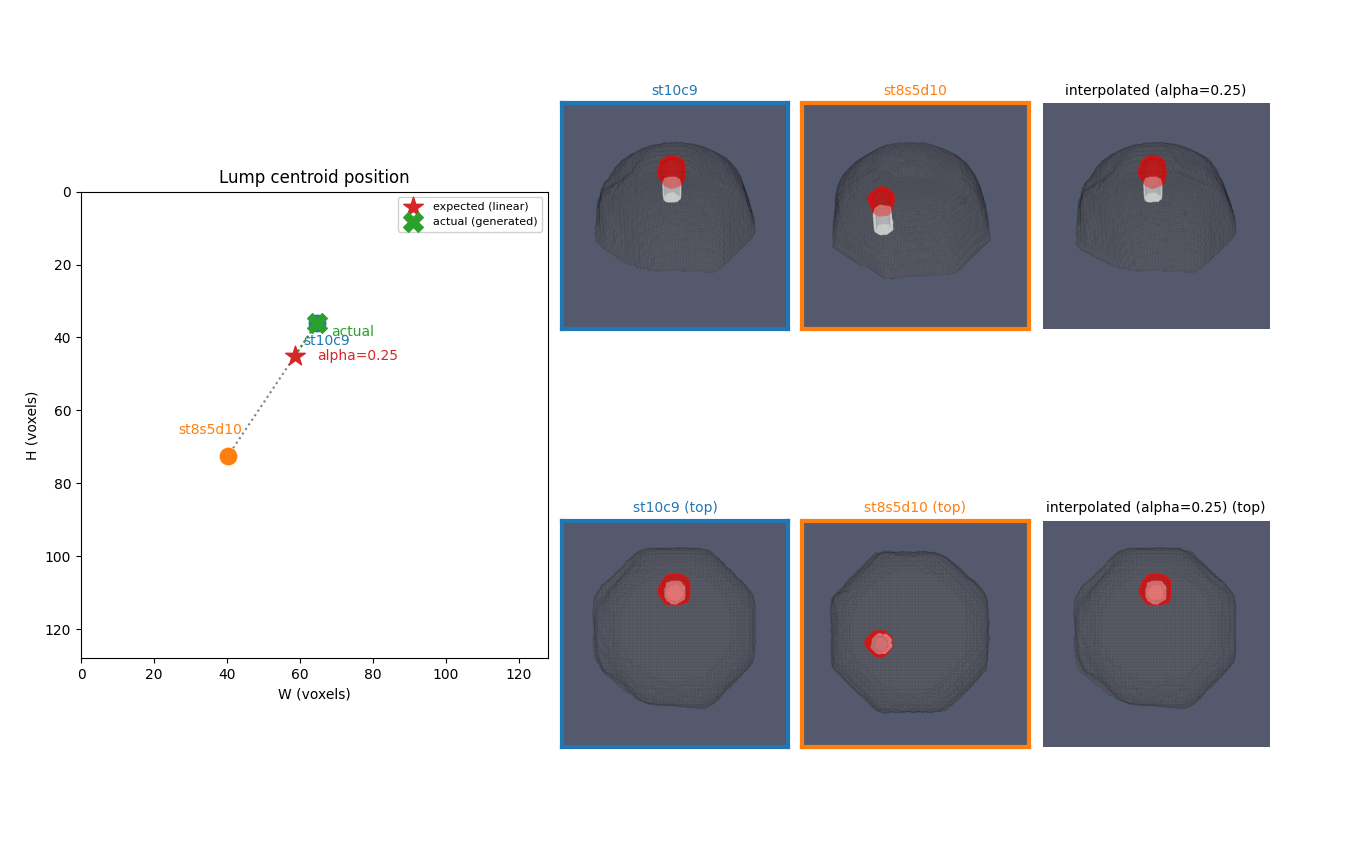
\includegraphics[width=0.48\textwidth]{imgs/summary/tmid_snap_alpha025.png}
\hfill
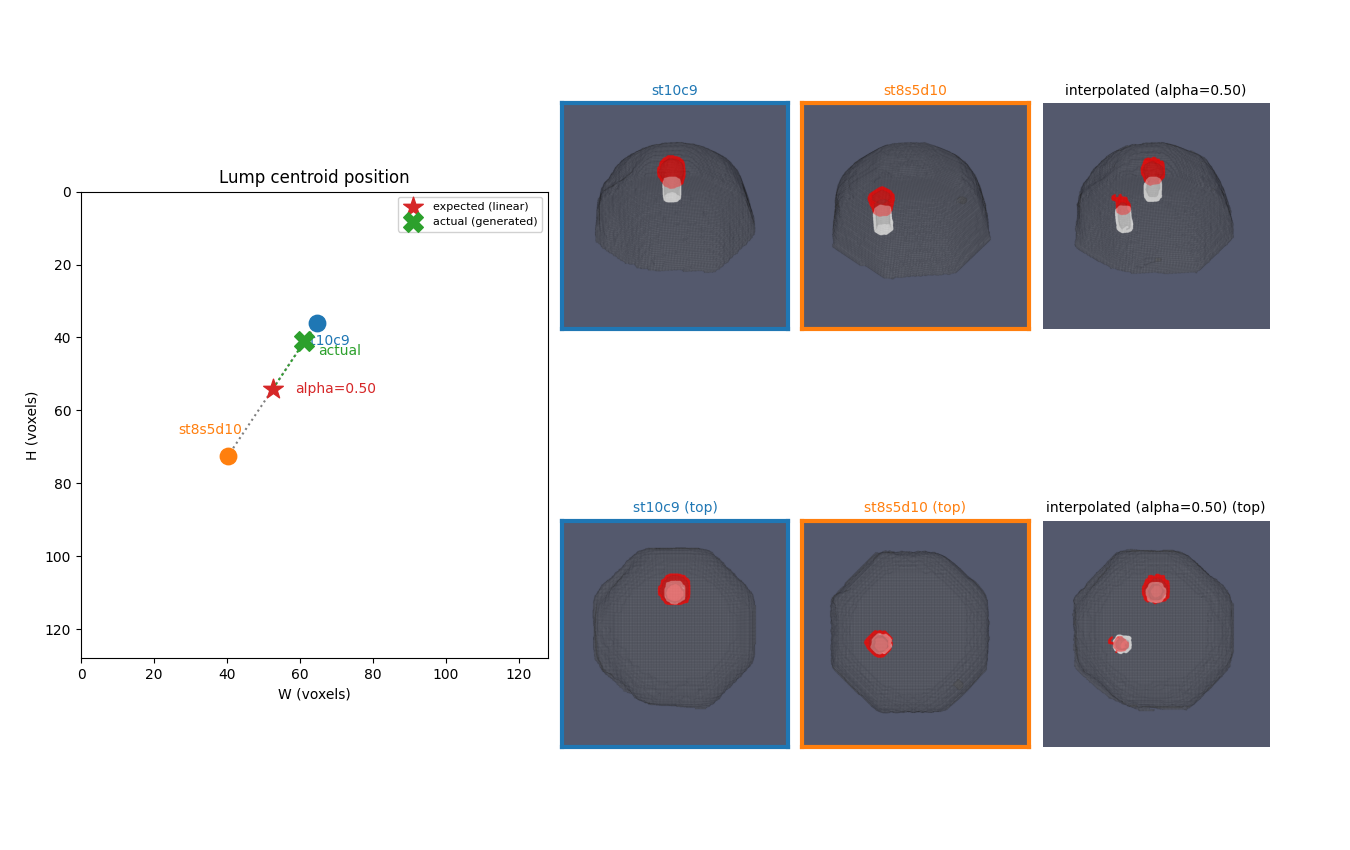
\includegraphics[width=0.48\textwidth]{imgs/summary/tmid_snap_alpha050.png}
\caption{Same pair (\texttt{st10c9} $\leftrightarrow$ \texttt{st8s5d10}), $t_{\text{mid}}=0.5$.
Left, $\alpha=0.25$: the output matches phantom A almost exactly (compare lump/pillar position
to the \texttt{st10c9} panel) rather than showing a 25\% blend toward B. Right, $\alpha=0.5$:
both A's and B's lumps appear simultaneously (visible as two separate red regions in the
top-down row) instead of one blended lump partway between them.}
\label{fig:tmid-snap}
\end{figure}

This means the model is not smoothly interpolating at any $t_{\text{mid}}$ tested --- it is
behaving like a nearest-neighbor selector in angle: close to A's specific trained direction it
reproduces A, close to B's it reproduces B, and exactly at the ambiguous midpoint it produces
a superposition of both rather than a genuinely new, blended anatomy. This directly explains
why ``avg\_lump\_components'' never drops cleanly to 1 anywhere in the table: at $\alpha=0.5$
specifically, 2 lumps (one from each endpoint) is close to the \emph{expected} outcome of this
snapping behavior, not evidence of a single well-formed interpolated lump. The centroid MAE
and fragmentation improvements at higher $t_{\text{mid}}$ are real, but they measure ``looks
closer to one of the two real endpoints, less torn than a full inversion would produce''
rather than ``genuinely interpolates between them.'' $t_{\text{mid}}$ narrows \emph{where}
the model breaks down, but does not fix the underlying issue described in Section~6 and
Section~4.4: the network was only ever taught the translation \emph{at} each individual real
phantom, never in the neighborhood between two of them --- and that remains true regardless
of how far back either endpoint is inverted before combining them. The more fundamental fix
proposed above (a compact, KL-regularized latent space) attacks that root cause directly;
$t_{\text{mid}}$, as tested here, does not.

\hsec{Other directions worth trying next}
$t_{\text{mid}}$ narrows \emph{where} the model breaks, but Section~8 showed it doesn't touch
\emph{why}. Four candidate next steps, roughly cheapest/least-certain to most
involved/most-targeted:

\hsub{1. Zero retraining: multi-hop interpolation through real neighbors}
Instead of interpolating directly between two arbitrary real phantoms --- one long hop across
a space where, per Section~4.5, $\sim\!10^3$ training points cover a vanishing sliver of
$d\approx1.7\times10^6$ dimensions --- build a similarity graph over the real phantoms (e.g.\
by noise-space or lump-position distance) and, for a chosen pair $A,B$, find a chain of
intermediate real phantoms connecting them. Interpolate each short hop instead of one long
jump, so every step only ever traverses the neighborhood of two real, well-covered points.
This needs no retraining at all --- purely a change to which pairs get interpolated and how
many steps, testable immediately with the existing pipeline. Trade-off: with only 40 case
IDs the neighbor graph is sparse, so this only helps pairs that already have plausible
intermediate real phantoms between them, and does nothing for the underlying issue when two
phantoms are simply far apart with nothing real in between.

\hsub{2. New training data: synthetic in-between supervision}
Nothing in training currently supervises the region between two real phantoms' paths. Fix
that directly: for pairs of real phantoms, compute an offline, geometrically-motivated
``halfway anatomy'' and add it as an auxiliary training target at intermediate points along
that pair's path. A standard way to build that target is per-class signed-distance-field
interpolation: for two binary masks $m_A, m_B$ of the same class, let $\mathrm{SDF}(m)$ be the
signed distance transform (negative inside the shape, positive outside, magnitude equal to
distance from the boundary). Then
\begin{equation}
\mathrm{SDF}_\alpha = (1-\alpha)\,\mathrm{SDF}(m_A) + \alpha\,\mathrm{SDF}(m_B), \qquad
m_\alpha = \mathbb{1}\big[\mathrm{SDF}_\alpha \le 0\big]
\end{equation}
gives a smoothly-morphing synthetic mask at any $\alpha$, per class, that can be turned into a
one-hot label volume and used as an extra regression target for $v_\theta$ near the
corresponding point on the $A$--$B$ path. This is the only option here that places real
supervision in the exact spot proven broken in Sections~4.5 and 8. Trade-off: the SDF-blended
target is a geometric heuristic, not verified ground truth (no real scan of a genuine
intermediate phantom exists), and it requires modifying the training loop and retraining, not
just a one-off inference-time experiment.

\hsub{3. Add the compression back: a compact, learned latent space}
Covered in full in Section~7: train a VAE-style encoder first, then run flow matching inside
its compact, KL-regularized latent space instead of the raw $d\approx1.7\times10^6$-dimensional
voxel space (the idea behind Latent Diffusion / Stable Diffusion). This is the most direct fix
for the root cause named in Section~4.4 --- no bottleneck currently means nothing forces the
noise space to be smoothly organized --- but it is also the largest change of the four: a new
model component to train, and no guarantee it converges cleanly on a dataset this small.

\hsub{4. Smoothness regularization on the velocity field}
A middle ground between (2) and (3): add a cheap penalty term during training that pushes
$v_\theta$ to respond similarly to slightly perturbed points, not only to points that lie
exactly on a trained path. Concretely, for a training point $x_t$, sample a small perturbation
$\epsilon \sim \mathcal{N}(0,\sigma^2 I)$ with $\sigma$ small relative to the typical shell
radius (Eq.~\eqref{eq:norm-mean}), and add
\begin{equation}
\mathcal{L}_{\text{smooth}} = \lambda \,\mathbb{E}\big[\, \|v_\theta(x_t + \epsilon, t) - v_\theta(x_t, t)\|^2 \,\big]
\end{equation}
to the training loss, with $\lambda$ a small weight. This is a one-line addition to the
training loop, no new data required. Trade-off: it only encourages smoothness in an
infinitesimal neighborhood of trained points, not that the large-scale neighborhood
\emph{between} two far-apart real phantoms --- which is what interpolation actually needs ---
becomes meaningful. Likely necessary but not sufficient on its own.

\hsec{Summary of concrete changes made this session}
\begin{itemize}[nosep]
\item Added class-weighted flow-matching loss (Eq.~\eqref{eq:weighted-loss}--\eqref{eq:weights}).
\item Added multi-pair, randomly-rotated real and noise interpolation with denser alpha sweeps.
\item Added a top-down render alongside the default angled view for every figure.
\item Color-coded each endpoint's render border to match its point on the position schematic.
\item Added the actual-vs-expected lump centroid diagnostic (Figure~\ref{fig:interp-broken}).
\item Built \texttt{visualize\_inversion.py} for the before~$\to z\to$~after figure (Figure~\ref{fig:inversion0}).
\item Fixed a concurrent-rendering corruption bug and a concurrent-checkpoint-overwrite bug.
\item Ran round-trip and step-count diagnostics to isolate the interpolation failure's cause.
\item Worked out the dimensionality/distribution analysis in Section~4, quantitatively
  explaining both the linear-vs-slerp choice and the $z$-rendering size mismatch.
\item Extended \texttt{ode.py} to support partial inversion/sampling at an arbitrary $t$, and
  built \texttt{sweep\_tmid.py} to test the $t_{\text{mid}}$ idea across $t_{\text{mid}} \in
  [0.1, 0.9]$ on 20 pairs with quantitative metrics (Section~8).
\item Discovered, by inspecting rendered examples rather than trusting the aggregate metrics
  alone, that the model snaps to whichever endpoint $\alpha$ is closer to instead of smoothly
  interpolating, at every $t_{\text{mid}}$ tested (Figure~\ref{fig:tmid-snap}) --- the real
  bottleneck is not $t_{\text{mid}}$, it is the lack of a compact, smoothly-organized latent
  space (Section~7).
\item Documented four candidate next directions, from a zero-retraining experiment to
  training-data and architecture changes (Section~9).
\end{itemize}

\end{document}
